\documentclass[aspectratio=169,xcolor=dvipsnames]{beamer}
\usetheme{SimplePlus}

% Links
\usepackage{hyperref}
\hypersetup{
    colorlinks=true,
    linkcolor=blue,
    filecolor=magenta,      
    urlcolor=brown,
    linkbordercolor=1 1 1,
    citebordercolor=1 1 1,
    linkbordercolor=1 1 1,
    menubordercolor=1 1 1,
    urlbordercolor=1 1 1,
}

% images
\usepackage{graphicx} 

%
\usepackage{booktabs} % Allows the use of \toprule, \midrule and \bottomrule in tables


\title[short title]{\textbf{Robot Mazes}} 
\subtitle{Project I Checkpoint - Artificial Inteligence}

\author[Marcelo  Francisco] {\textbf{Grupo 21} \\ \begin{tabular}{r l} 
	\email{up201906086@up.pt} & Marcelo Henriques Couto \\
	\email{up201907361@up.pt} & Francisco Pinto de Oliveira \\
\end{tabular}
}

\institute[FEUP] 
{
    Faculdade de Engenharia da Universidade do Porto
}
\date{\today} 



\begin{document}

\begin{frame}
    \titlepage
\end{frame}


\begin{frame}{Problem Description}
    Implement an Artificial Inteligence agent based on heuristic search methods to solve \href{https://erich-friedman.github.io/puzzle/robot/}{Robot Mazes} puzzle. 

    \vspace{0.5em}

    \begin{minipage}{0.62\textwidth}
        \begin{itemize}
            \item \textbf{Grid:} The puzzle is made up of a 5x5 grid, with a start and finish positions. Between each spot in the grid, there can be a wall.
            \item \textbf{Robot and Movement:} The robot is placed at the starting spot and can make a limited number of movements (Left, Right, Up or Down), depending on the puzzle. When there are no moves left, he will repeat the sequence chosen until he gets stuck or reaches the ending spot.
        \end{itemize}
    \end{minipage}%
    \begin{minipage}{0.38\textwidth}
        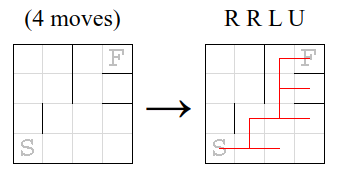
\includegraphics[width=50mm]{img/puzzle.png}
    \end{minipage}
    \begin{itemize}
            \item \textbf{Objective:} The objective is to, for a given puzzle, decide the correct sequence of movements for the robot to loop from start to finish.
    \end{itemize}
\end{frame}

\begin{frame}{Related Work}
    \begin{itemize}
        \item \textbf{\href{https://moodle.up.pt/pluginfile.php/196597/mod_resource/content/0/ArtificialIntelligence_ModernApproach_3rdEdition.pdf}{Artificial Intelligence: A Modern Approach 3rd Edition:}} Search algorithm implementation
        \item \textbf{\href{https://towardsdatascience.com/escape-the-maze-with-a-search-algorithm-bb0f1cf876e0}{Escape the Maze with A* Search Algorithm: }} Help with heuristic discovery
    \end{itemize}
\end{frame}


\begin{frame}{Problem Formulation as a Search Problem}
    \textbf{State Representation:} With N being the number of moves allowed, state S is an array of size N of the movements chosen. \\
    \textbf{Initial State:} A random state. E.g. S = [Right,Up,Left,Down] \\
    \textbf{Objective Test:} The cycle of movements of the given state, repeated indefinitely, always changes position after an iteration and eventually reaches the goal spot. \\
    \textbf{Operators:}
    \begin{table}
        \begin{tabular}{l l l l}
            \toprule
            \textbf{Operator} & \textbf{Pre-Condition} & \textbf{Effect} & \textbf{Cost} \\
            \midrule
            ChangeMov(i,m)  & $ i >= 0 \land i < N \land S[i] \neq m $ & $S[i] = m $  & 1 \\
            \bottomrule
        \end{tabular}
        \caption{Operators}
    \end{table}
    
    With this approach, we consider every solution to be equally optimal, being the speed of the algorithm the desirable aspect to optimize.
\end{frame}




\begin{frame}{Implementation}
    \textbf{Language:} Python \\
    \textbf{Environment:} Anaconda \\
    \textbf{Dependencies:} pygame, pygame\_menu \\
    \textbf{Data Structures:} 
    \begin{enumerate}
        \item Map representing the positions of the walls in the maze - python \textit{dictionary}
        \item List representing the movements of the robot in sequence (state) - python \textit{list}
    \end{enumerate}\\
    \textbf{Algorithms:} Simulation of a given sequence of movements (state)\\
\end{frame}


\end{document}